%
% rewriting open objects
% a motivating example
%

% --- comment out when compiling ---
%%
%	rewriting open objects
%	style
%	

%
%  packages
%

\usepackage{amsfonts}
\usepackage{amssymb}  
\usepackage{amsthm} 
\usepackage{amsmath} 
\usepackage{caption}
\usepackage[inline]{enumitem}
	\setlist{itemsep=0em, topsep=0em, parsep=0em}
	\setlist[enumerate]{label=(\alph*)}
\usepackage{doi}
\usepackage{etoolbox}
\usepackage[]{hyperref}
%	\definecolor{hyperrefcolor}{rgb}{0,0,0.7}
	\hypersetup{colorlinks,linkcolor={blue},citecolor={blue},urlcolor={blue}}
\usepackage{graphicx}
	\graphicspath{ {images/} }
\usepackage{mathtools}
\usepackage[numbers]{natbib}
\usepackage{stmaryrd} 
\usepackage{subcaption}
\usepackage{subfiles}
\usepackage{tikz}
	\usetikzlibrary{matrix,arrows,shapes,decorations.markings,decorations.pathreplacing}
\usepackage{todonotes}
\usepackage{url}
\usepackage{xcolor}

%
% commands
%

\newcommand{\RR}{\mathbb{R}}
\newcommand{\ZZ}{\mathbb{Z}}
\newcommand{\NN}{\mathbb{N}}
\newcommand{\QQ}{\mathbb{Q}}
\newcommand{\CC}{\mathbb{C}}
\newcommand{\DD}{\mathbb{D}}
\newcommand{\MM}{\mathbb{M}}
\renewcommand{\epsilon}{\varepsilon}

\newcommand{\Set}{\cat{Set}}
\newcommand{\Graph}{\cat{Graph}}
\newcommand{\RGraph}{\cat{RGraph}}
\newcommand{\Top}{\cat{Top}}
\newcommand{\Cat}{\cat{Cat}}
\newcommand{\A}{\cat{A}}
\newcommand{\B}{\cat{B}}
\newcommand{\C}{\cat{C}}
\newcommand{\X}{\cat{X}}
\newcommand{\Y}{\cat{Y}}
\newcommand{\Z}{\cat{Z}}
\newcommand{\core}[1]{\mathbf{core}(#1)}

\newcommand{\defn}[1]{\textbf{#1}}
\newcommand{\op}[1]{\operatorname{#1}}
\newcommand{\cat}[1]{\mathbf{#1}}
\newcommand{\dblcat}[1]{\mathbb{#1}}
\renewcommand{\t}[1]{\text{#1}}


\newcommand{\from}{\colon}
\newcommand{\xto}[1]{\xrightarrow{#1}}
\newcommand{\sm}{\smallsetminus}
\newcommand{\tospan}{\xrightarrow{\mathit{sp}}}
\newcommand{\tocospan}{\xrightarrow{\mathit{csp}}}
\newcommand{\diagram}[1]{\raisebox{-0.5\height}{\includegraphics{#1}}}

\newcommand{\Sp}[1]{\mathbf{Sp}(#1)}
\newcommand{\MonSp}[1]{\mathbf{MonSp}(#1)}
\newcommand{\SSp}[1]{\mathbb{S}\mathbf{p}(#1)}
\newcommand{\Csp}[1]{\mathbf{Csp}(#1)}
\newcommand{\CCsp}[1]{\mathbb{C}\mathbf{sp}(#1)}
\newcommand{\SpSp}[1]{\mathbf{Sp}(\mathbf{Sp}(#1))}
\newcommand{\SSpSp}[1]{\mathbb{S}\mathbf{p(\mathbf{Sp}(#1))}}
\newcommand{\CspCsp}[1]{\mathbf{Csp}(\mathbf{Csp}(#1))}
\newcommand{\CCspCsp}[1]{\mathbb{C}\mathbf{sp}(\mathbf{Csp}(#1))}
\newcommand{\MonSpCsp}[1]{\mathbf{MonicSp}(\mathbf{Csp}(#1))}
\newcommand{\MMonSpCsp}[1]{\mathbb{M}\mathbf{onicSp}(\mathbf{Csp}(#1))}
\newcommand{\EpCspSp}[1]{\mathbf{EpicCsp}(\mathbf{Csp}(#1))}
\newcommand{\EEpCspSp}[1]{\mathbb{E}\mathbf{picCsp}(\mathbf{Sp}(#1))}
\newcommand{\SpCsp}[1]{\mathbf{Sp}(\mathbf{Csp}(#1))}
\newcommand{\SSpCsp}[1]{\mathbb{S}\mathbf{p}(\mathbf{Csp}(#1))}

\newcommand{\FuncCsp}[1]{ #1 \t{-} \mathbf{Csp}}
\newcommand{\OpenOb}[1]{ #1 \t{-} \mathbf{Open} }
\newcommand{\Rewrite}[1]{ #1 \t{-} \mathbf{Rewrite} }
\newcommand{\RRewrite}[1]{ #1 \t{-} \mathbb{R}\mathbf{ewrite} }
\newcommand{\MonRewrite}[1]{ #1 \t{-} \mathbf{MonRewrite} }
\newcommand{\MMonRewrite}[1]{ #1 \t{-} \mathbb{M}\mathbf{on}\mathbb{R}\mathbf{ewrite} }

%
% math operators
%

\DeclareMathOperator{\Hom}{Hom}
\DeclareMathOperator{\id}{id}
\DeclareMathOperator{\ob}{Ob}
\DeclareMathOperator{\arr}{arr}
\DeclareMathOperator{\im}{im}
\DeclareMathOperator{\Aut}{Aut}
\DeclareMathOperator{\Bij}{Bij}
\DeclareMathOperator{\Sub}{Sub}
\DeclareMathOperator{\colim}{colim}

%
% envirnments and counters
%

\newtheorem{thm}{Theorem}[section]
\newtheorem{lem}[thm]{Lemma}
\newtheorem{prop}[thm]{Proposition}
\newtheorem{cor}[thm]{Corollary}

\theoremstyle{remark}
	\newtheorem{remark}[thm]{Remark}
	\newtheorem{notation}[thm]{Notation}

\theoremstyle{definition}
	\newtheorem{ex}[thm]{Example} 
	\newtheorem{df}[thm]{Definition}

% \setcounter{tocdepth}{1} % Sets depth for table of contents. 

%
% tikz types
%
\tikzset{->-/.style={decoration={%
			markings,
			mark=at position .5 with {\arrow{>}}},postaction={decorate}}
}
\tikzset{->-pos/.style={decoration={%
			markings,
			mark=at position #1 with {\arrow{>}}},postaction={decorate}}
}
\tikzset{->-/.style={decoration={%
			markings,
			mark=at position .5 with {\arrow{>}}},postaction={decorate}}
}
\tikzset{->-pos/.style={decoration={%
			markings,
			mark=at position #1 with {\arrow{>}}},postaction={decorate}}
}

%
% inline diagrams
%
\newcommand{\rgraph}[2]{%
	$\begin{tikzpicture}
	\node (a) at (0,0) {$ #1 $};
	\node (b) at (1,0) {$ #2 $};
	\draw [->] (a.30) to (b.150);
	\draw [->] (a.-30) to (b.-150);
	\draw [->] (b) to (a);
	\end{tikzpicture}$
}
\newcommand{\graph}[2]{%
	$\begin{tikzpicture}
	\node (a) at (0,0) {$ #1 $};
	\node (b) at (1,0) {$ #2 $};
	\draw [->] (a.30) to (b.150);
	\draw [->] (a.-30) to (b.-150);
	\end{tikzpicture}$
} % input preamble
%\bibliography{} % input bibliograph	

\section{A motivating example} 
\label{sec:MotivatingExample}

This section serves two functions. First, we discuss the example that motivates this paper.  Within our discussion, we take the opportunity to set both notation and language used in the sequel.  

When reading network theory literature written from the compositional perspective, one comes across the notion of an open graph. 
	\todo{cite}
The level of formality this definition is given varies between authors, but the core idea is that an \emph{open graph} is a $ \Set $-diagram $ E \rightrightarrows N $ together with a subset $ \partial \subseteq N$ equipped with a partition $ \partial = \partial_{ \t{in} } + \partial_{ \t{out} } $.
	\todo{insert diagram D1-open graph}
The conceit is that the subset of nodes $ \partial $ is a boundary that is accessible to other open graphs. Elements of $ \partial_{ \t{in} } $ and $ \partial_{ \t{out} } $ are thought of as inputs and outputs, respectively.  Given two open graphs $ (E \rightrightarrows N , \partial_{ \t{in} } + \partial_{ \t{out} }) $ and $ (E' \rightrightarrows N' , \partial'_{ \t{in} } + \partial'_{ \t{out} }) $, such that $ \partial_{ \t{out} } = \partial'_{ \t{in} } $, then we can construct the graph $ (E + E' \rightrightarrows (N + N') / \partial_{ \t{out} } = \partial'_{ \t{in} } ,  \partial_{ \t{in} } + \partial'_{ \t{out} } ) $.  For example,
	\todo{insert diagram D2-glueing open graphs}.
We casually add that by appropriately modifying the definition of a graph morphism, one can define a morphism of open graphs.

A primary motivation behind this construction is to model the process of connecting networks together.  Although, some networks contain additional information that cannot be conveyed by an open graph as described above.
	\todo{cite examples: circ, zx-calc, petri nets, etc}
To accommodate such demands, we generalize the notion of an open graph to that of an \emph{open object} and develop some basic theory for open objects.  

One feature that distinguishes this work from other related work is our preference for reflexive graphs over directed graphs.  Before mentioning our reasons, let us clarify exactly what we mean by these two sorts of graphs. Denote by $ \rgraph{\bullet}{\bullet} $ the category with two objects $ [0] $ and $ [1] $ with two arrows $ s,t \from [1] \to [0] $ and an arrow $ r \from [0] \to [1] $ that is a section to both $ s $ and $ t $.  Throughout this text, the category of reflexive graphs is $ \RGraph \coloneqq [ \rgraph{\bullet}{\bullet} , \Set] $ and the category of directed graphs is $ \Graph \coloneqq [ \graph{\bullet}{\bullet} , \Set ] $.  The reasons for working with reflexive graphs are myriad.  For one, elements $ 1 \to \Gamma $ of a graph $ \Gamma $ are not just nodes, but nodes with a loop attached.  It follows that the underlying nodes functor $ \RGraph \to \Set $ is representable by the terminal graph. This is not the case for the underlying nodes functor of type $ \Graph \to \Set $.  Also, the objects of $ \RGraph $ are truncated simplicial sets. The advantage of this goes, perhaps, beyond the scope of this paper. Suffice to say, when working with graph relations, particularly those homotopical in nature, we desire a well-known model structure to work with.  Having said this, let it be known that from this point, any reference to a ``graph'' will mean a ``reflexive graph'' unless specified otherwise. This includes cases when we modify ``graph'' with an adjective. For instance, by ``open graph'' we actually mean ``open reflexive graph''.

Recall that the terms ``discrete'' and ``codiscrete'' usually refer to the, respectively, left and right adjoints of a global sections functor. We will use these terms a bit more loosely here.  Namely, given a functor $ \A \to \X $ forgetting structure,
	\todo{is this right?}
we call a left adjoint \textbf{discrete} and a right adjoint \textbf{codiscrete}, assuming their existence.  For example, the functor $ \Set \to \RGraph $ sending given by sending a set $ x $ to the graph $ \rgraph{x}{x} $ with only the required loops is the discrete graphs functor, as it is left adjoint to $ \RGraph (1,-) $.  Also, the functor $ \Set \to \RGraph $ sending a set to the complete graph is the codiscrete functor, as it is right adjoint to $ \RGraph (1,-) $.

Because open graphs are the archetypal example of an open object, it behooves us to formalize that which we have so far glossed over. 

\begin{df} \label{df:OpenGraph}
	Let $ \partial \from \Set \to \RGraph $ be the discrete graph functor.  An \textbf{open graph} is a cospan of the form $ \partial x \to \gamma \gets \partial y $.  
\end{df}

Immediately, there emerges two perspectives on open graphs, both alluded to above. The first is that we want to be able to glue together suitable open graphs to form new open graphs. This leads one to consider a category with open graphs $ \partial x \to \gamma \gets \partial y $ as arrows from $ \partial x $ to $ \partial y b $.  As we discuss below in further detail, composition of such arrows uses pushouts. Heuristically, this can be thought of as a ``categorical gluing''.  The second perspective is that open graphs are mathematical objects which deserve their own morphisms.  Indeed, a morphism 
\[
(\partial x \to \gamma \gets \partial y) \to ( \partial x' \to \gamma' \gets \partial y' )
\]
of open graphs is a triple $ (f,g,h) $ that fits into a commuting diagram
\[
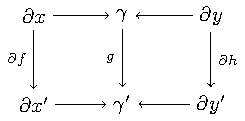
\includegraphics{diag_open-graph-morph_reopn}
\]
This leads to another category where open graphs are objects, as opposed to arrows.  

Having two categories featuring open graphs---one as arrows, the other as objects---one thinks to construct a double category containing all of this structure.  In fact, we do this in Section BLAH. 
	\todo{input appropriate section}
In the following section, we generalize open graphs to `open objects' and construct a pair of categories, one with open objects as arrows and the other with open objects as objects.  




